\documentclass[handout]{beamer}

\usepackage[utf8]{inputenc} % Language and font encoding
\usepackage[icelandic]{babel}
\usepackage[T1]{fontenc}


\usepackage{tikz}
\usepackage[listings,theorems]{tcolorbox}
\usepackage{booktabs}
\usepackage{minted} %Minted and configuration
\usemintedstyle{default}

\renewcommand{\theFancyVerbLine}{\sffamily \arabic{FancyVerbLine}}
%%%%%%%%%%%
% More math
%%%%%%%%%%%
\newcommand{\Mod}[1]{\ \text{mod}\ #1}

%%%%%%%%%%%%%%%%%%%%%%
% Beamer configuration
%%%%%%%%%%%%%%%%%%%%%%
\setbeamertemplate{navigation symbols}{}
\usecolortheme{dove}
\setbeamercolor{frametitle}{fg=white}

\usebackgroundtemplate%
{%
\vbox to \paperheight{

\includegraphics[width=\paperwidth]{Pics/hi-slide-head-2016}

\vfill
\hspace{0.5cm}
\includegraphics[width=0.3\paperwidth]{Pics/hi-von-logo}
\vspace{0.4cm}
    }%
}

\AtBeginSection[]
{
  \begin{frame}<beamer>
    \frametitle{Yfirlit}
    \tableofcontents[currentsection]
  \end{frame}
}

\setbeamerfont{frametitle}{size=\normalsize}
\addtobeamertemplate{frametitle}{}{\vspace*{0.5cm}}

%%%%%%%%%%%%%%%%%%%%%%%%%
% tcolorbox configuration
%%%%%%%%%%%%%%%%%%%%%%%%%

% Setup from: http://tex.stackexchange.com/a/43329/21638
\tcbset{%
    noparskip,
    colback=gray!10, %background color of the box
    colframe=gray!40, %color of frame and title background
    coltext=black, %color of body text
    coltitle=black, %color of title text 
    fonttitle=\bfseries,
    alerted/.style={coltitle=red, colframe=gray!40},
    example/.style={coltitle=black, colframe=green!20, colback=green!5},
}


%%%%%%%%%%%%%%%%%%%%%%%
% Further configuration
%%%%%%%%%%%%%%%%%%%%%%%
\hypersetup{colorlinks=true,pdfauthor={Eirikur Ernir Thorsteinsson},linkcolor=blue,urlcolor=blue}
\graphicspath{{./Pics/}}

\author{Eiríkur Ernir Þorsteinsson}
\institute{Háskóli Íslands}
\date{Haust 2016}

\title{Stærðfræðimynstur í tölvunarfræði}
\subtitle{Vika 8, seinni fyrirlestur}

\begin{document}

\begin{frame}
\titlepage
\end{frame}


\section{Inngangur}

\begin{frame}{Í síðasta tíma}
\begin{itemize}
 \item Miðmisseriskönnun
 \item Talning og rakningarvensl
 \item Kvik bestun
\end{itemize}
\end{frame}

\section{Lausnir á rakningarvenslum}

\begin{frame}{Lausnir á rakningarvenslum}
\begin{itemize}
 \item Hingað til höfum við leyst rakningarvensl með því að skoða fyrstu liðina í runu sem uppfyllir venslin og sjá mynstur
 \item Við getum gert aðeins betur, en til þess þurfum við betri skilgreiningar
\end{itemize}
\end{frame}

\begin{frame}{Skilgreining}
\begin{tcolorbox}[title=Línuleg einsleit rakningarvensl með fastastuðlum]
Línuleg einsleit rakningarvensl (e. \emph{a linear homogeneous recurrence relation}) af stigi $k$ með fastastuðla eru rakningarvensl á eftirfarandi sniði:
\[
 a_n = c_1 a_{n-1} + c_2a_{n-2} + \ldots + c_ka_{n-k}
\]
þar sem $c_1, c_2, \ldots, c_k$ eru rauntölur, með $c_k \neq 0$.
\end{tcolorbox}
\begin{itemize}
 \item Rakningarvenslin eru línuleg af því hægri hlið jöfnunnar er einföld summa af fyrri liðum
 \item Rakningarvenslin eru einsleit því allir liðir hægri hliðarinnar eru fast margfeldi einhvers $a_j$
\end{itemize}
\end{frame}

\begin{frame}{Dæmi}
\begin{itemize}[<+->]
 \item Hvert er stig línulegu einsleitu rakningarvenslanna $P_n = 1.11P_{n-1}$?
 \begin{itemize}
  \item Stigið er 1, hver liður veltur á einum fyrri lið
 \end{itemize}
 \item Hvert er stig línulegu einsleitu rakningarvenslanna $f_n = f_{n-1} + f_{n-2}$?
 \begin{itemize}
  \item Stigið er 2
 \end{itemize}
 \item Hvert er stig línulegu einsleitu rakningarvenslanna\\ $a_n = a_{n-5}$?
 \begin{itemize}
  \item Stigið er 5
 \end{itemize}
\end{itemize}
\end{frame}

\begin{frame}{Dæmi}
\begin{itemize}[<+->]
 \item Hvert er stig línulegu einsleitu rakningarvenslanna $P_n = 1.11P_{n-1}$?
 \begin{itemize}
  \item Stigið er 1, hver liður veltur á einum fyrri lið
 \end{itemize}
 \item Hvert er stig línulegu einsleitu rakningarvenslanna $f_n = f_{n-1} + f_{n-2}$?
 \begin{itemize}
  \item Stigið er 2
 \end{itemize}
 \item Hvert er stig línulegu einsleitu rakningarvenslanna\\ $a_n = a_{n-5}$?
 \begin{itemize}
  \item Stigið er 5
 \end{itemize}
\end{itemize}
\end{frame}

\begin{frame}{Dæmi}
\begin{itemize}
 \item Nokkur rakningarvensl sem eru ekki línuleg einsleit rakningarvensl með fastastuðla
 \begin{itemize}[<+->]
  \item $a_n = a_{n-1} + a_{n-2}^2$
  \begin{itemize}
   \item ekki línuleg
  \end{itemize}
  \item $H_n = 2H_{n-1} + 1$
  \begin{itemize}
   \item Ekki einsleit
  \end{itemize}
  \item $B_n = nB_{n-1}$
  \begin{itemize}
   \item Ekki með fastastuðla
  \end{itemize}
 \end{itemize}
\end{itemize}
\end{frame}

\begin{frame}{Að finna lausnir}
Þegar við leitum að runu sem á að uppfylla línuleg einsleit rakningarvensl með fastastuðla erum við venjulega að leita að runu með liði á sniðinu $a_n = r^n$, þar sem $r$ er fasti. Athugum að runa með $a_n = r^n$ er lausn á venslunum $ a_n = c_1 a_{n-1} + \ldots + c_ka_{n-k}$ ef og aðeins ef
\[
 r^n = c_1r^{n-1} + c_2r^{n-2} + \ldots + c_kr^{n-k}
\]
sem er jafngilt
\[
 r^k - c_1r^{k-1} - c_2r^{k-2} - \ldots - c_{k-1}r - c_k = 0
\]
. Við köllum síðustu jöfnuna kennijöfnu (e. \emph{characteristic equation}) rakningarvenslanna.
\end{frame}

\begin{frame}{Setning}
Skoðum sérstaklega lausnir á línulegum einsleitum rakningarvenslum af stigi 2:
\begin{tcolorbox}[title=Lausn einfaldra rakningarvensla af stigi 2]
Látum $c_1$ og $c_2$ vera rauntölur og að $r^2 - c_1r - c_2 = 0$ hafi tvær aðskildar rætur $r_1$ og $r_2$. Þá er runan $\{a_n\}$ lausn á rakningarvenslunum $a_n = c_1a_{n-1} + c_2a_{n-2}$ ef og aðeins ef $a_n = \alpha_1r_1^n + \alpha_2r^n_2$ fyrir $n=0,1,2,\ldots$ og $\alpha_1$ og $\alpha_2$ eru fastar.
\end{tcolorbox}

\end{frame}

\begin{frame}{Dæmi}
Getum við fundið lausn á rakningarvenslunum $a_n = a_{n-1} + 2a_{n-2}$ með upphafsskilyrðin $a_0 = 2$ og $a_1 = 7$? \pause

\vspace{0.5cm}
Já. Kennijafna rakningarvenslanna er $r^2 - r - 2 = 0$, með rætur $r_1 = 2$ og $r_2 = -1$. Þá er runan lausn á rakningarvenslunum ef og aðeins ef $a_n = \alpha_12^n + \alpha_2(-1)^n$ fyrir einhverja fasta $\alpha_1$ og $\alpha_2$.\pause

Upphafsskilyrðin gefa $a_0 = 2 = \alpha_1 + \alpha_2$ og $a_1 = 7 = \alpha_12 + \alpha_2(-1)$. Leysum þær og fáum $\alpha_1 = 3$ og $\alpha_2 = -1$. Þá er $\{a_n\}$ með

\[
 a_n = 3 \cdot 2^n - (-1)^n
\]
lausn á rakningarvenslunum.

\end{frame}

\begin{frame}{Dæmi: Fibonacci}
Finnum formúlu fyrir $n$-tu Fibonacci-töluna. \pause

$n$-ta Fibonacci-talan er gefin með $f_n = f_{n-1} + f_{n-2}$, sem hefur kennijöfnuna $r^2 - r - 1 = 0$ með ræturnar 
\[r_1 = \frac{1 + \sqrt{5}}{2} \]
og
\[r_2 = \frac{1 - \sqrt{5}}{2}\]
svo
\[
 f_n = \alpha_1\left(\frac{1 + \sqrt{5}}{2}\right)^n + \alpha_2\left(\frac{1 - \sqrt{5}}{2}\right)^n
\]
\end{frame}

\begin{frame}{Dæmi: Fibonacci}
Reiknum $\alpha_1$ og $\alpha_2$ út frá upphafsskilyrðunum $f_0 = 0$ og $f_1 = 1$:
\begin{align*}
f_0 &= \alpha_1 + \alpha_2 = 0\\
f_1 &= \alpha_1\left(\frac{1 + \sqrt{5}}{2}\right) + \alpha_2\left(\frac{1 - \sqrt{5}}{2}\right) = 1
\end{align*}
og fáum $\alpha_1 = \frac{1}{\sqrt{5}}$, $\alpha_2 = -\frac{1}{\sqrt{5}}$, svo
\[
 f_n = \frac{1}{\sqrt{5}}\left(\frac{1 + \sqrt{5}}{2}\right)^n -\frac{1}{\sqrt{5}}\left(\frac{1 - \sqrt{5}}{2}\right)^n
\]
\end{frame}

\begin{frame}{Fleiri setningar}
\begin{itemize}
 \item Setningin á fyrri glæru á einungis við línuleg einsleit rakningarvensl af stigi 2 með aðskildar rætur
 \begin{itemize}
  \item Það er ekki sérlega almennt
 \end{itemize}
 \item Í kafla 8.2 höfum við einnig\ldots
 \begin{itemize}
  \item setningu um línuleg einsleit rakningarvensl af stigi 2 með eina rót (Theorem 2)
  \item setningu um línuleg einsleit rakningarvensl af stigi $k$ með $k$ aðskildar rætur (Theorem 3)
  \item setningu um línuleg einsleit rakningarvensl af stigi $k$ með rætur sem geta verið endurteknar (Theorem 4)
 \end{itemize}
\end{itemize}
\end{frame}

\begin{frame}{Almennari setning}
\begin{columns}
\column{0.25\textwidth}
{\small
Fyrir hverja rót $r$ í kennijöfnunni er stuðullinn margliða af stigi $m - 1$, þar sem $m$ er fjöldi skipta sem rótin kemur fyrir.
}
\column{0.75\textwidth}
\begin{center}
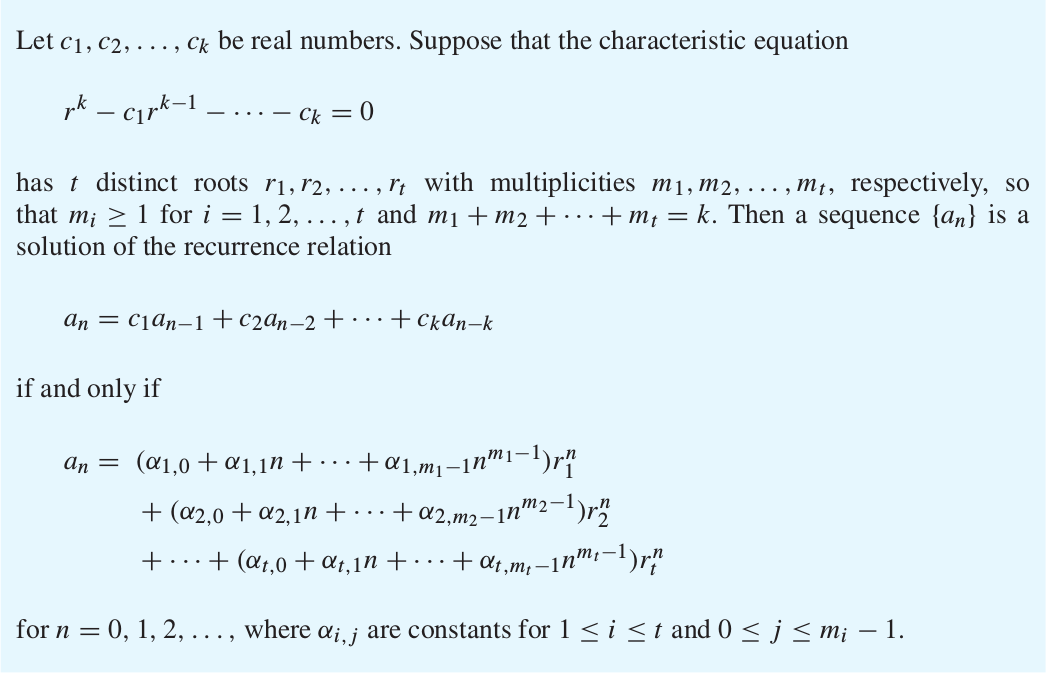
\includegraphics[width=\textwidth]{solving-recurrence}
\end{center}
\end{columns}
\end{frame}

\begin{frame}{Fleiri gerðir rakningarvensla}
Við getum líka sett fram setningar um lausnir á óeinsleitum (e. \emph{nonhomogeneous}) línulegum rakningarvenslum með fastastuðla. Slík rakningarvensl eru á sniðinu 
\[
 a_n = c_1 a_{n-1} + c_2a_{n-2} + \ldots + c_ka_{n-k} + F(n)
\]
þar sem $F(n)$ er fall sem ekki er núll. Einsleitu rakningarvenslin $a_n = c_1 a_{n-1} + c_2a_{n-2} + \ldots + c_ka_{n-k}$ eru kölluð tilsvarandi einsleitu rakningarvenslin.
\end{frame}

\begin{frame}{Óeinsleit rakningarvensl}
Getum sett fram setningu um óeinsleit rakningarvensl
\begin{center}
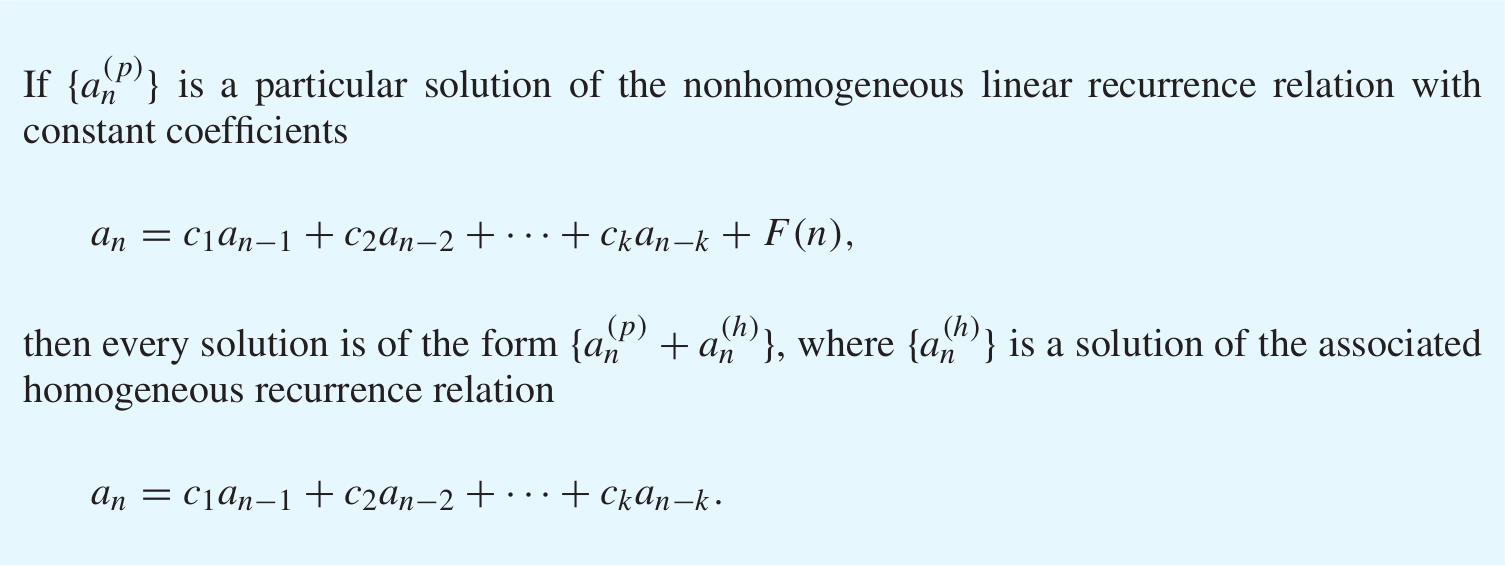
\includegraphics[width=\textwidth]{solving-nonhomo-recurrence}
\end{center}
Lausn á óeinsleitum rakningarvenslum er sem sagt summa lausnar á einsleitu rakningarvenslunum og sérlausnar á óeinsleitu r-venslunum.
\end{frame}

\begin{frame}{Dæmi}
Lítum á Example 10 í kafla 8.2 í kennslubók.
\end{frame}



\section{Deila-og drottna reiknirit}

\begin{frame}{Deila-og-drottna reiknirit}
\begin{itemize}
 \item Mörg endurkvæm reiknirit fylgja svokallaðri deila-og-drottna (e. \emph{divide-and-conquer}) aðferðafræði
 \begin{itemize}
  \item Þau \emph{deila} vandamálinu niður í smærri tilvik af sjálfu sér
  \item Þau \emph{drottna} (yfir?) vandamálinu með því að nota smáu lausnirnar
 \end{itemize}
 \item Við getum notað rakningarvensl til að kanna tímaflækjur deila-og-drottna reiknirita
\end{itemize}
\end{frame}

\begin{frame}{Helmingunarleit}
\begin{itemize}
 \item Skoðum fjölda samanburða sem við þurfum að framkvæma í helmingunarleit í $n$ staka runu
 \item Hvert skref í helmingunarleit minnkar stærð leitarbils úr $n$ niður í $\frac{n}{2}$ (ef $n$ er slétt)
 \item Í hverju skrefi framkvæmum við tvo samanburði
 \begin{itemize}
  \item Einn til að sjá hvorn helming rununnar við skoðum næst
  \item Einn til að sjá hvort við séum búin
 \end{itemize}
 \item Sé $b(n)$ fjöldi samanburða sem við þurfum til að leita að staki í runu af lengd $n$ fáum við þá
\end{itemize}
\[
 b(n) = b(n/2) + 2
\]
\end{frame}

\begin{frame}{Merge sort}
\begin{itemize}
 \item Merge sort skiptir runu af lengd $n$ sem raða skal endurtekið í hlutrunur af lengd $n/2$
 \begin{itemize}
  \item Síðan eru minna en $n$ samanburðir notaðir til að sameina hlutrunurnar tvær
 \end{itemize}
 \item Þá getum við lýst fjölda samanburða sem þarf til að raða $n$ staka runu með merge sort með fallinu $M(n)$,
\end{itemize}
\[
 M(n) = 2M(n/2) + n
\]
\end{frame}

\begin{frame}{Setning}
\begin{center}
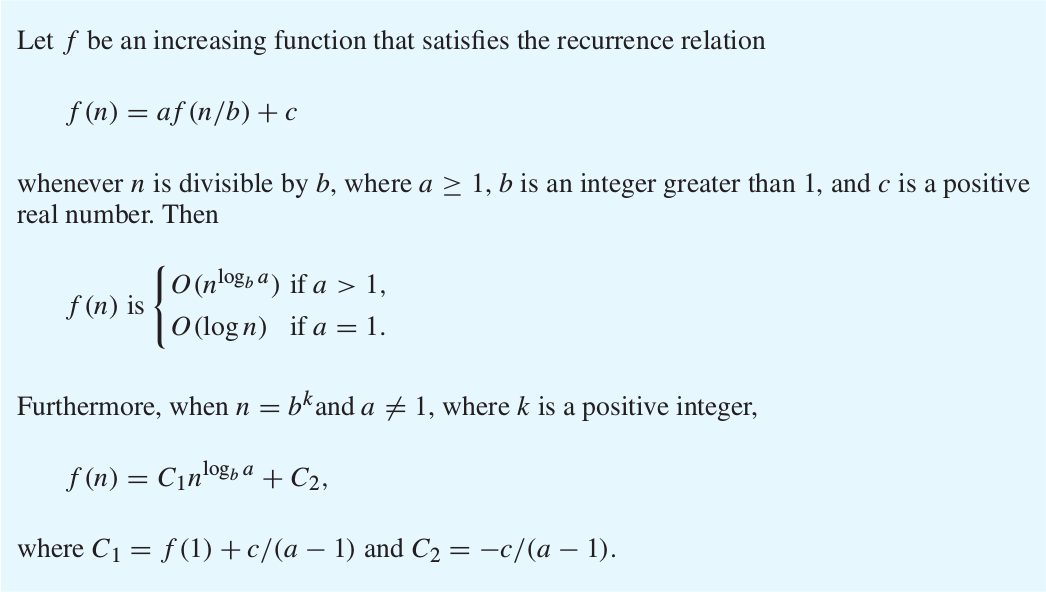
\includegraphics[width=\textwidth]{divide-and-conquer-time}
\end{center}
\end{frame}

\begin{frame}{Dæmi}
Fjöldi samanburða í helmingunarleit var $b(n) = b(n/2) + 2$ þegar $n$ er slétt tala. Hver er tímaflækja helmingunarleitar á stóra-O sniði? \pause

\vspace{1cm}
Skoðum setningu á fyrri glæru. Hér er $a=1$ svo helmingunarleit er $O(\log(n))$ reiknirit, sem passar við fyrri áætlanir.
\end{frame}

\begin{frame}{Öflugri setning}
Til að finna tímaflækjur reiknirita á borð við merge sort þurfum við öflugri setningu. Slík setning er:

\begin{center}
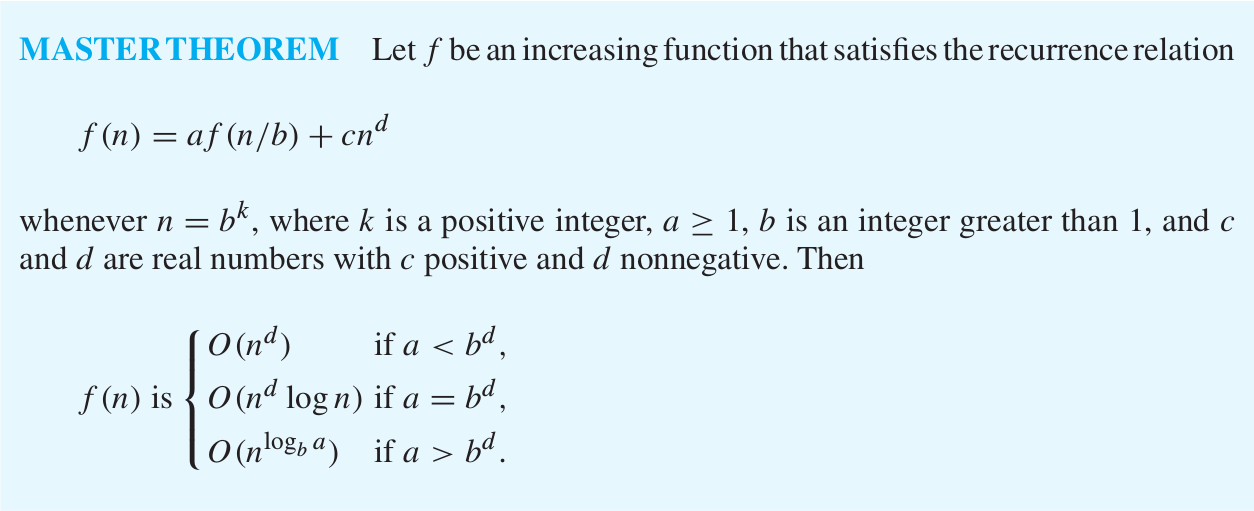
\includegraphics[width=\textwidth]{master-theorem}
\end{center}
\end{frame}

\begin{frame}{Dæmi}
Fjöldi samanburða í merge sort var $M(n) = 2M(n/2) + n$. Notum ``master theorem'' til að finna tímaflækju á stóra-O sniði.

\vspace{1cm}
Berum saman við $f(n) = af(n/b) + cn^d$ í master theorem. Sjáum að fallið sem lýsir fjölda samanburða passar sé $b=2$, $c=1$, $d=1$, $a=2=b^d$, svo við fáum að tímaflækjan sé $O(n^d\log (n)) = O(n\log(n))$ sem passar við fyrri áætlanir.
\end{frame}

\begin{frame}{Næst}
Vensl (9.1 og e.t.v 9.2)
\end{frame}



\end{document}
